A natural way according to the mantra presented by \citeauthor{Shneiderman1996} to visualise a dataset is to start with an overview. This supports the user's understanding of the complexity and size of the whole dataset. However giving an overview first is also dependant on the dataset. Imagine a \ac{GIS} like OpenStreetMap\footnote{See \href{https://www.openstreetmap.org}{https://www.openstreetmap.org}} would show random location, e.g. a valley with a lot of detail as a starting point. There are two contrary use cases where such a starting point would make sense or not.
\begin{enumerate}
\item If the dataset the map is based on only contains data of that specific ``random'' valley shown, it definitely makes sense to only show that valley. The dataset does not contain information about all valleys, therefore making it unnecessary to show the whole map of the earth as an overview first.
\item The use case mentioned already, implicitly explains a bad use case of a random starting point. If a dataset inheres structure, like a whole map of the world, it is not useful to start at a specific location, therefore showing an overview of the earth first makes more sense.
\end{enumerate}

Focus and context describes a concept that puts a specific part of dataset, called subset, in focus while still showing an overview of the other part. One example implementation of this concept are fisheye views, originally developed by \citeauthor{Furnas:1986} \iacite{Furnas:1986}. Figure \ref{fig:focus} on page \pageref{fig:focus} shows a modern implementation of the focus and context concept based on a fisheye view. The focus in this Figure is set somewhere between the blue and orange circle in the middle of the Figure. This part is magnified as one can see on the circle size, while the ones further away are smaller and a little distorted.

\begin{figure}[!htb]
\centering
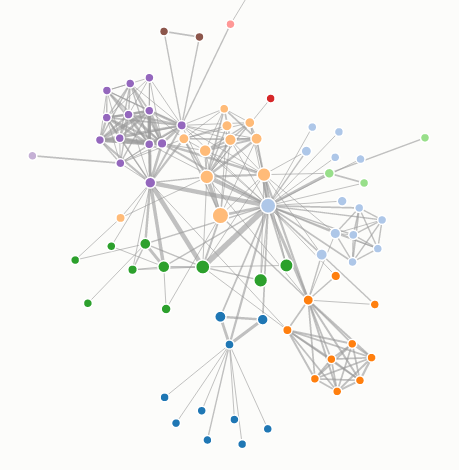
\includegraphics[height=5cm,keepaspectratio]{images/methods/interaction/focus.png}
\caption[
    The focus and context concept based implemented with a fisheye view, Urldate: 07.2016 \newline
    \small\texttt{\url{https://bost.ocks.org/mike/fisheye/}}.
]{The focus and context concept implemented with a fisheye view. The blue node in the center of the Figure and the yellow node left to it are bigger compared to the other ones. This is due to the magnification of this part.}
\label{fig:focus}
\end{figure}

\citeauthor{Kosara2003} categorise the aforementioned method as distortion-oriented \iacite{Kosara2003}. Other techniques they list are summarised below:
\newpage
\begin{description}
\item[Overview methods] show the context in a separate layer in the same place \iacite{Kosara2003}.
\item[Filtering] shows additional information of particular subparts e.g. with a magic lens. They provide an object of any shape that can move freely. The area it covers is shown with more information \iacite{Bier:1993}.
\item[In-Place techniques] are similar to filtering without the requirement of a lens. The implementation of the technique points out information to the user, e.g. by highlighting. The program can also take the initiative and point the user to interesting data \iacite{Kosara2003}.
\end{description}
